
\chapter{Simulazioni}

Le simulazioni presentate in questo capitolo si concentrano prevalentemente sulla molecola di idruro di litio (LiH), scelta per la sua struttura di piccole dimensioni e per il numero contenuto ridotto di orbitali elettronici coinvolti, che la rendono un sistema ideale per testare metodi quantistici. In particolare, è stata calcolata l’energia dello stato fondamentale al variare della distanza internucleare, con l’obiettivo di tracciare il profilo del potenziale elettronico. In LiH, il minimo di energia si colloca attorno a $1.595$ \AA, in accordo con dati sperimentali disponibili in letteratura \cite{LiH_nist}. I dettagli relativi alle simulazioni, inclusi i codici utilizzati, sono consultabili e disponibili nella \inglese{repository} GitHub: \cite{AnsOME}.

% ==============================================================================================================
\section{Introduzione al codice}\label{sez:introduzione-codice}

In questa sezione viene descritto il codice utilizzato per le simulazioni, con particolare riferimento alla piattaforma offerta da Qiskit \cite{qiskit2024}, una delle piattaforme più diffuse per la programmazione quantistica. Qiskit fornisce strumenti avanzati per la creazione, simulazione e ottimizzazione di circuiti quantistici, fondamentali per affrontare problemi di chimica quantistica come la determinazione degli stati fondamentali e la simulazione di reazioni.

Si presenta una panoramica generale su come realizzare simulazioni tramite il Variational Quantum Eigensolver (VQE) in Qiskit, illustrando i passaggi essenziali e le scelte metodologiche chiave. Inoltre, vengono approfonditi alcuni concetti specifici, come la scelta delle basi e degli ottimizzatori, elementi centrali nella configurazione delle simulazioni quantistiche.
La selezione della base influenza direttamente la rappresentazione della molecola, determinando sia il numero di qubit richiesti che l’accuratezza dei risultati. Basi meno complesse, come la STO-3G, vengono spesso utilizzate per ridurre il costo computazionale, mentre basi più articolate, come la 6-31G, possono migliorare la precisione dei risultati a scapito di una maggiore complessità.
Gli ottimizzatori, d’altra parte, influenzano il processo di minimizzazione dell’energia e la velocità con cui si raggiunge la convergenza. A seconda del problema e delle caratteristiche della simulazione, è possibile scegliere tra diversi \inglese{optimizers} presto implementabili con Qiskit, come SPSA, COBYLA e SLSQP, ciascuno con vantaggi specifici per scenari diversi.


% --------------------------------------------------------------------------------------------------------------
\subsection{Impostazione del problema}

Il primo passo è implementare il sistema molecolare all'interno del codice attraverso \myinline{PySCFDriver}, che fa da ponte fra le classi di Qiskit e la libreria di chimica PySCF~\cite{pyscf}. Come argomenti si inseriscono gli attributi della molecola, quindi si esegue il metodo \myinline{.run()} per estrarre un \myinline{ElectronicStructureProblem}: oggetto che rappresenta il problema elettronico. 

% DRIVER ________________________________________________________
\begin{tcolorbox}[title=Dichiarazione molecola]
\begin{lstlisting}[language=Python]
LiH_geometry = f"""Li 0. 0. 0.; H 0. 0. {distance}"""

driver = PySCFDriver(
           atom   = LiH_geometry,
           basis  = 'sto3g',
           charge = 0,
           spin   = 0,
           unit   = DistanceUnit.ANGSTROM
         )

problem = driver.run()
\end{lstlisting}
\vspace{-0.2cm}
\end{tcolorbox}

Con \myinline{FreezeCoreTransformer} si possono congelare gli orbitali \inglese{core} della molecola, il che permette di ridurre la dimensione del problema con una piccola perdita di precisione dovuta all'approssimazione. Questo compromesso è generalmente considerato ragionevole, poiché il contributo degli orbitali esclusi diventa un semplice shift all'energia totale.

% PROBLEM _______________________________________________________
\begin{tcolorbox}[title=Congelamento orbitali core e hamiltoniana]
\begin{lstlisting}
fc_transformer = FreezeCoreTransformer()
fc_problem     = fc_transformer.transform(problem)
\end{lstlisting}
\vspace{-0.2cm}
\end{tcolorbox}

% ..............................................................................................................
\subsubsection{Scelta della base}

Ad oggi sono state introdotte numerose basi per rappresentare gli orbitali molecolari, alcune delle quali permettono di ottenere accuratezze elevate, anche se il costo computazionale cresce rapidamente all’aumentare del numero di orbitali atomici. Le basi STO-$n$G vengono principalmente impiegate per studi preliminari e approssimativi, mentre calcoli più dettagliati richiedono basi più articolate. Un esempio di queste è 6-31G, una base di tipo \inglese{split-valence} che combina sei funzioni gaussiane per il \inglese{core} e due serie di gaussiane per gli elettroni di valenza, migliorando la descrizione degli orbitali.

Di seguito è riportato il Grafico~\ref{fig:FCI-e-basi}, in cui si confrontano i risultati di FCI nelle basi STO-3G, STO-6G e 6-31G. 

\begin{figure}[H]
    \centering
    \hspace{-1cm}
    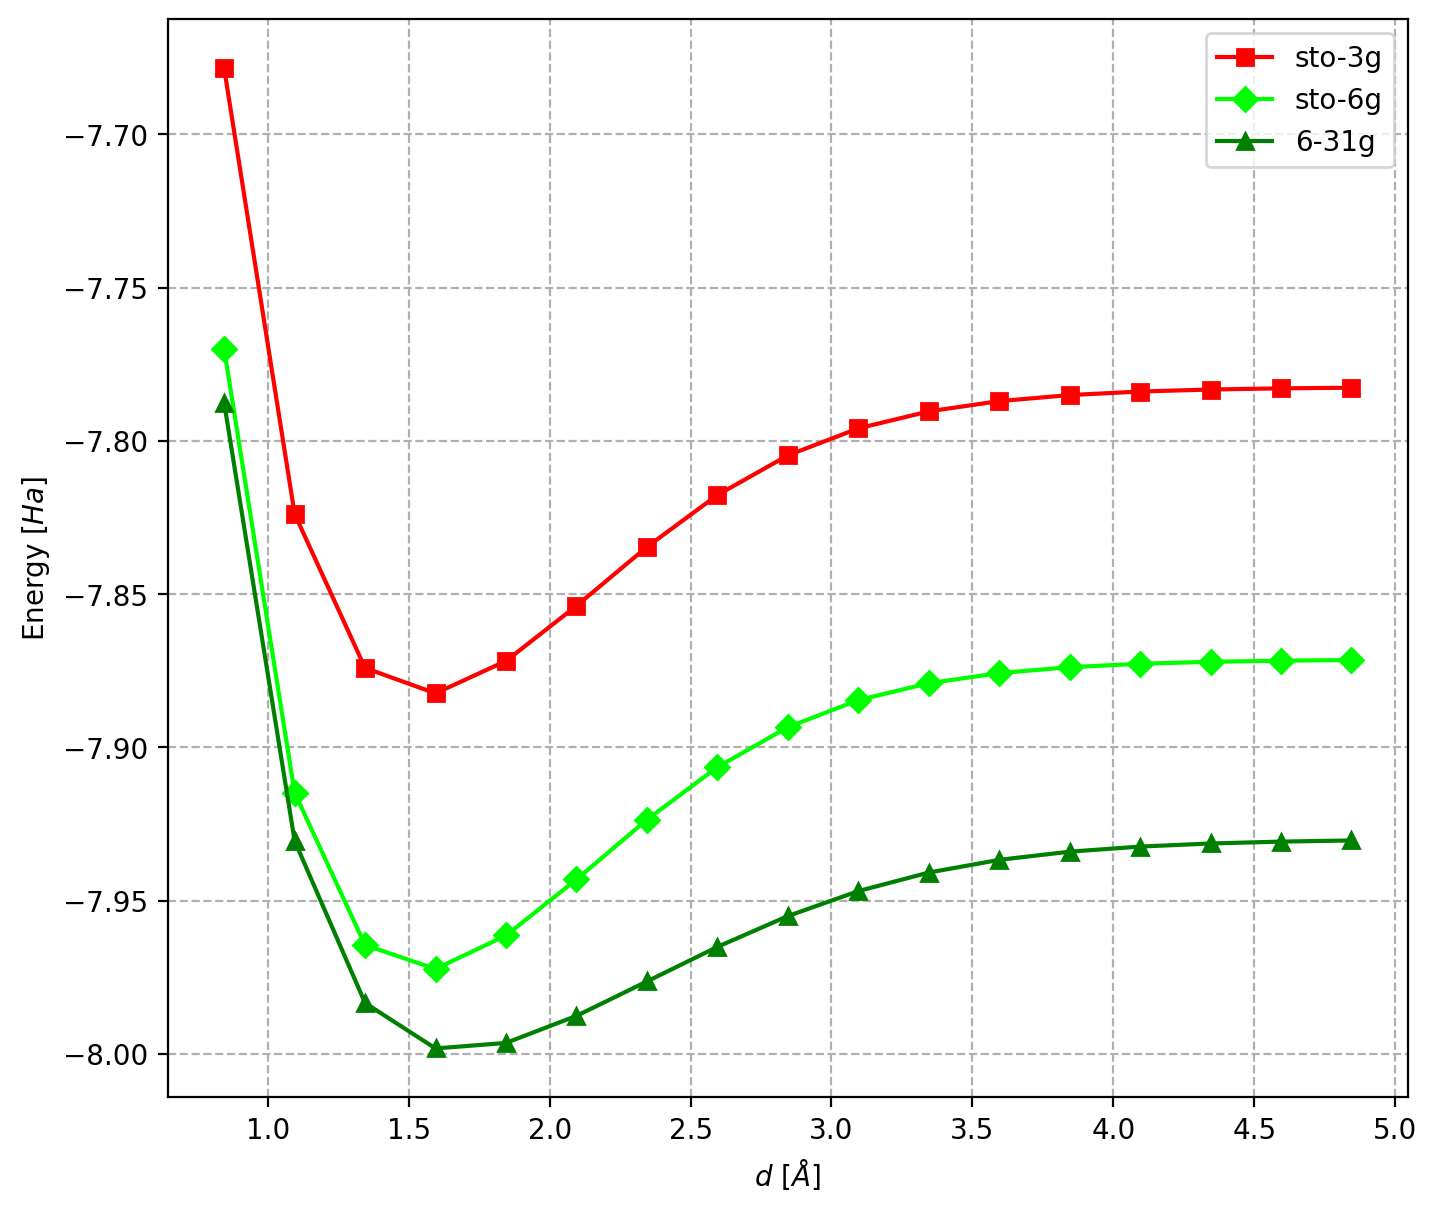
\includegraphics[width=.6\linewidth]{Immagini/Capitolo_3/FCI_e_basi.png}
    \caption{LiH: FCI con diverse basi.}
    \label{fig:FCI-e-basi}
\end{figure}

Le STO-$n$G sovrastimano l’energia in modo marcato ma richiedono tempi di calcolo notevolmente inferiori rispetto a 6-31G. In questo lavoro l’obiettivo è confrontare il costo di diversi circuiti quantistici, per cui è sufficiente lavorare con la base STO-3G.

\newpage

% --------------------------------------------------------------------------------------------------------------
\subsection{Ansatz}

\begin{minipage}{0.58\textwidth}
    Qiskit offre un'ampia scelta di ansatze UCC \cite{qiskit_UCC}, implementabili con poche righe di codice, qui sotto esemplificate per un generico ordine di eccitazioni~$X$. Si veda ad esempio il circuito $q$-UCCS, riportato qui a destra, generato dalla classe \myinline{UCCS} per le analisi della molecola di LiH. Innanzitutto, si può notare che la base STO-3G utilizzata per definire il problema dà luogo ad un circuito con 10 qubit, che per motivi di lunghezza viene suddiviso in quattro sezioni. 
    Come illustrato in Sezione~\ref{subsec:coupled-cluster}, la funzione d'onda \inglese{Coupled Cluster} è costruita a partire da uno stato di Hartree-Fock; i qubit 0 e 5, a cui vengono applicate delle rotazioni U, corrispondono agli stati occupati, mentre gli altri rappresentano orbitali \textbf{virtuali}. Dopodiché, si può osservare che i gate successivi sono applicati seguendo il \inglese{pattern} presentato in Figura~\ref{fig:eccitazioni-singole}, che mostrava l'insieme di operazioni necessarie per riprodurre le eccitazioni singole.
    È importante sottolineare che, tra i circuiti $q$-UCC utilizzati, $q$-UCCS è il meno costoso in termini di risorse, con $q$-UCCD e $q$-UCCSD che possono arrivare a profondità trenta volte maggiori. 
    

\end{minipage}
\begin{minipage}{0.42\textwidth}
    \begin{figure}[H]
        \centering
        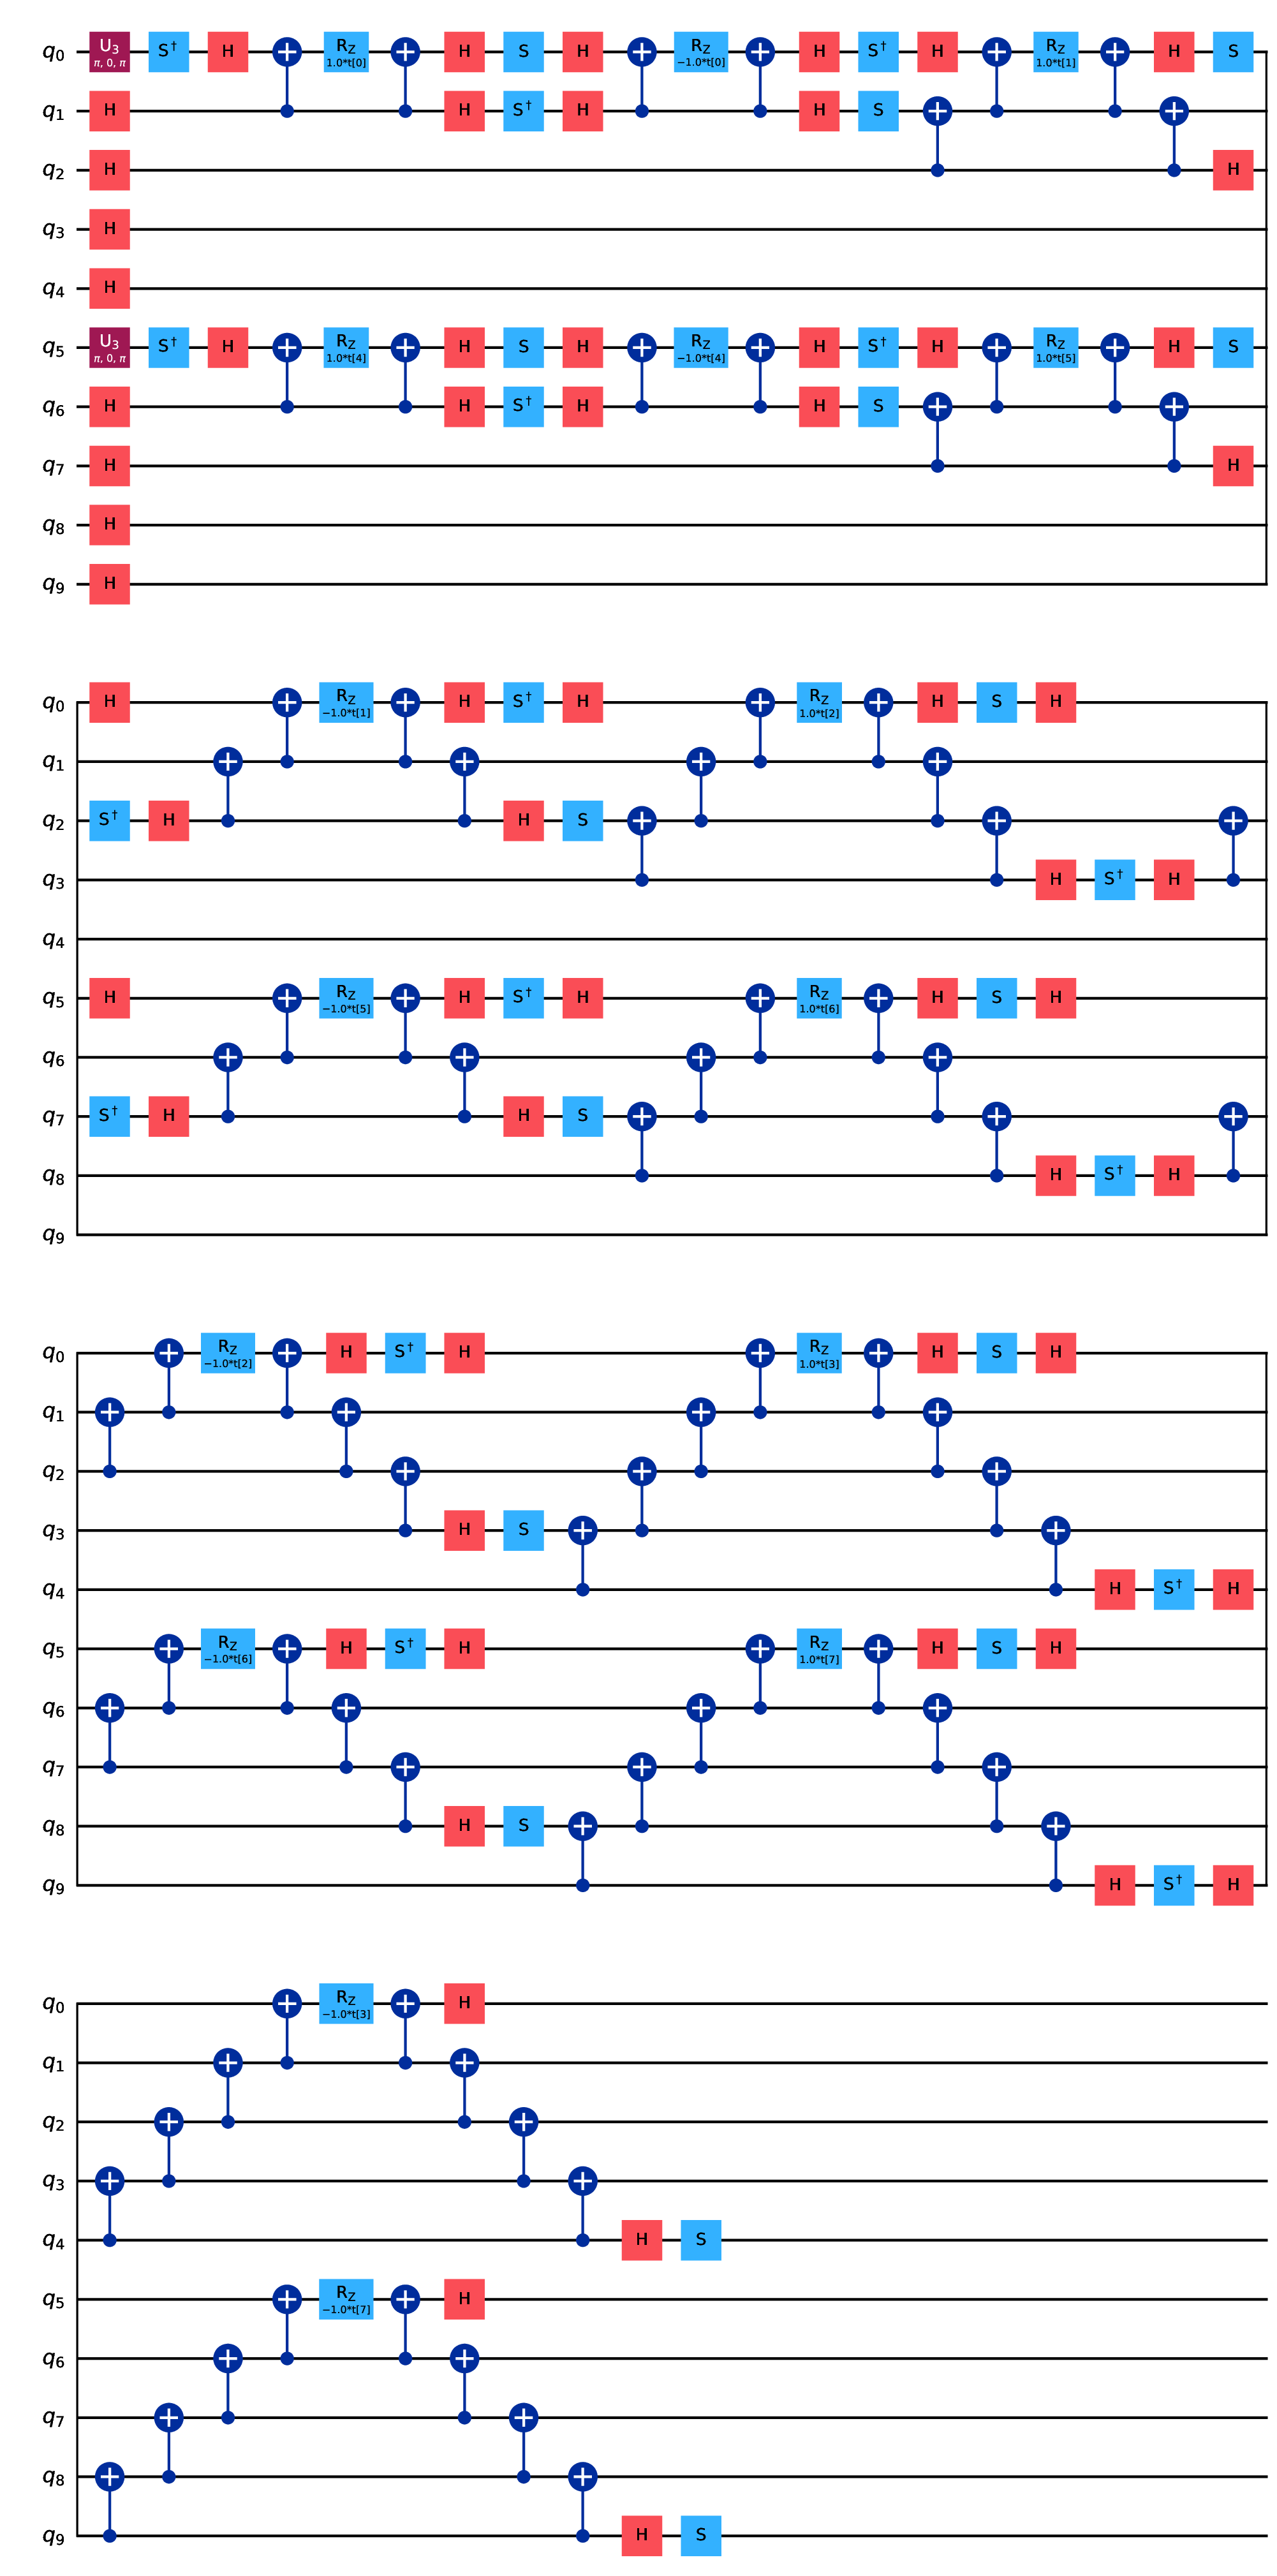
\includegraphics[width=\textwidth]{Immagini/Capitolo_3/uccs_circuit.png}
        \caption{Circuito UCCS.}
        \label{fig:circuito-uccs}
    \end{figure}
\end{minipage}

% ANSATZ UCC ____________________________________________________
\begin{tcolorbox}[title=Dichiarazione generico ansatz UCC$X$]
\begin{lstlisting}
uccx_qc = UCCX (
    fc_problem.num_spatial_orbitals,
    fc_problem.num_particles,
    mapper,
    excitations = 'x' # e.g.: 's', 'd', 'sd'
    initial_state=HartreeFock(
        fc_problem.num_spatial_orbitals,
        fc_problem.num_particles,
        mapper,
    ),
)

bounds = [[-np.pi,np.pi] for _ in range(uccx_qc.num_parameters)]
uccx_qc.parameter_bounds = bounds
\end{lstlisting}
\vspace{-0.2cm}
\end{tcolorbox}

Si noti che è necessario esplicitare un oggetto \myinline{mapper}, cioè il metodo di codifica da utilizzare per tradurre il problema in un circuito. Come discusso alla Sezione~\ref{subsec:qubit-mapping}, nelle simulazioni di questo elaborato si è utilizzato l'isomorfismo di Jordan-Wigner, espresso in Qiskit con la classe \myinline{JordanWignerMapper}.

L'ansatz rotazionale \inglese{hardware-efficient} invece viene implementato tramite la classe \myinline{EfficientSU2}, che può essere configurata con molta flessibilità:

% ANSATZ Efficient ______________________________________________
\begin{tcolorbox}[title=Dichiarazione ansatz hardware-efficient]
\begin{lstlisting}
efficient = EfficientSU2 (
    num_qubits, 
    reps=1,
    entanglement ='reverse_linear', 
    su2_gates=['ry', 'rz']
    initial_state=HartreeFock(
        fc_problem.num_spatial_orbitals,
        fc_problem.num_particles,
        mapper,
    ),
)

# stampo il circuito
efficient.draw('mpl')
\end{lstlisting}
\vspace{-0.5cm}
\begin{center}
    \hspace{-0.5cm}
    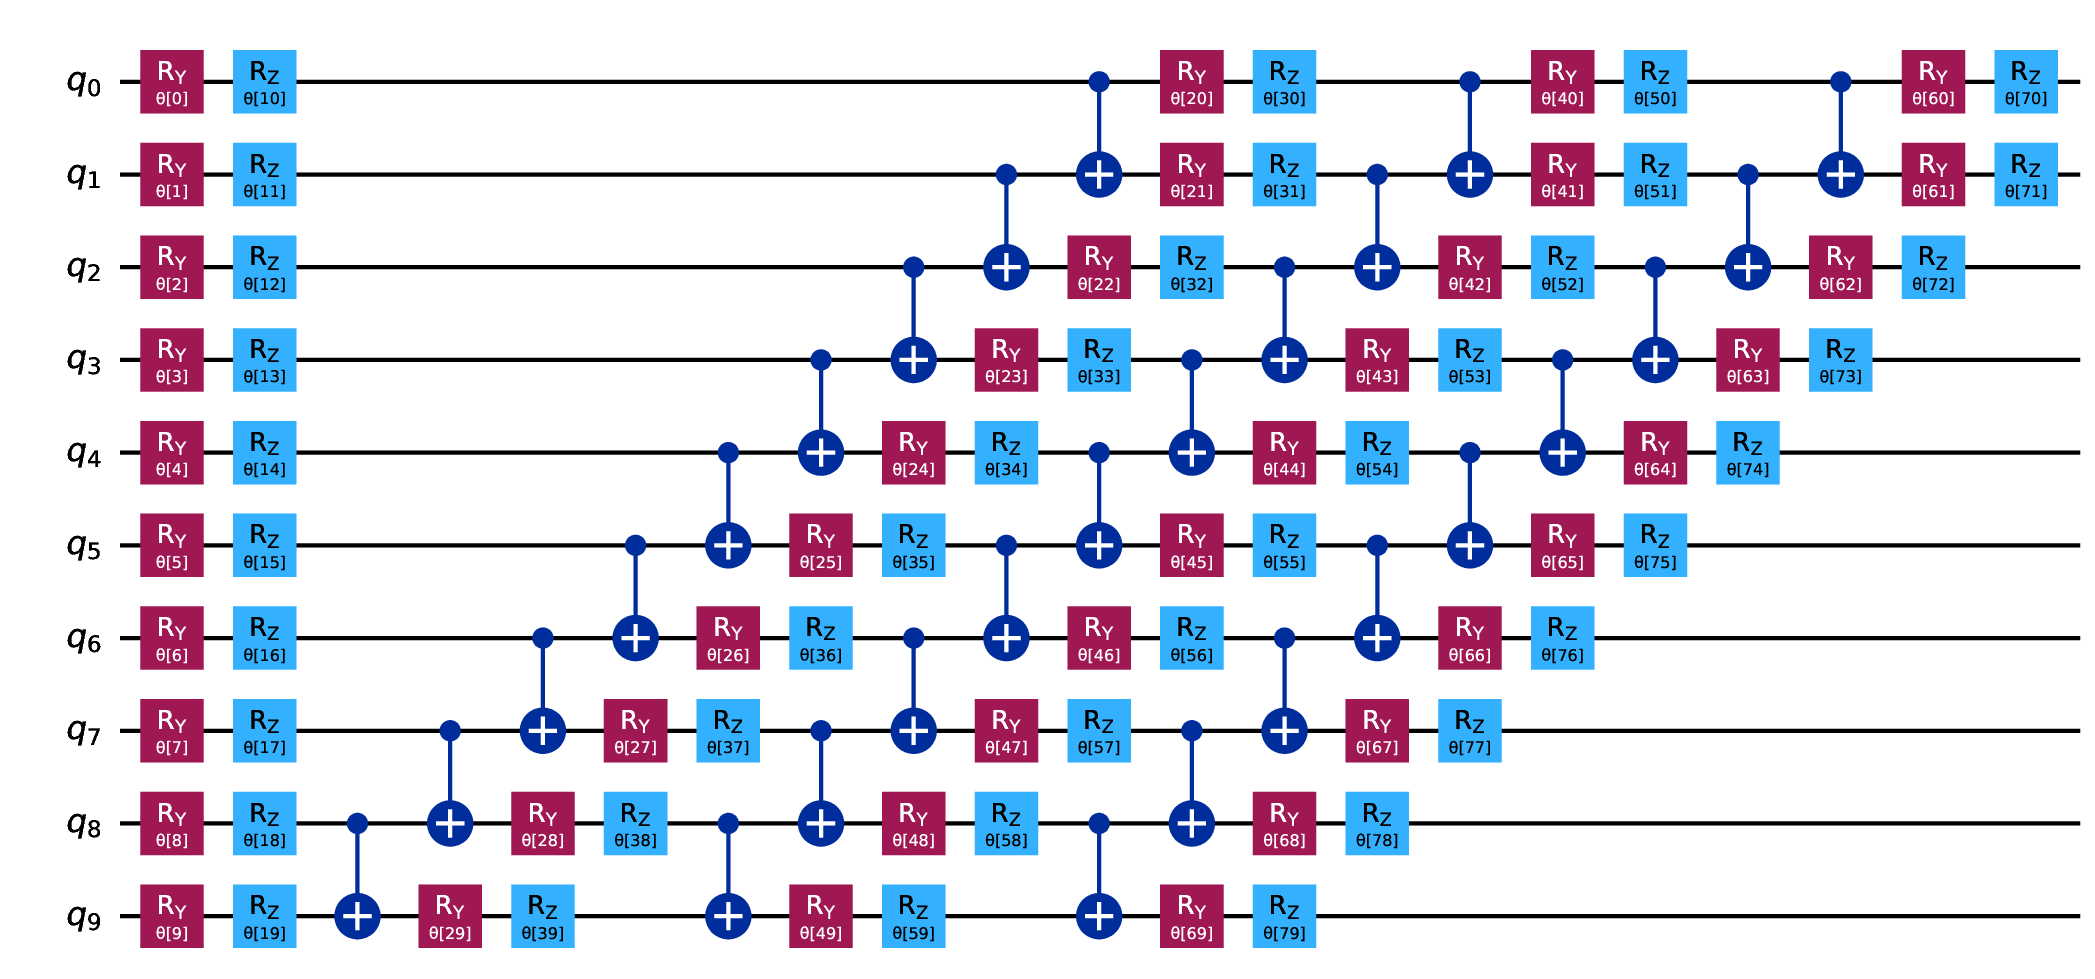
\includegraphics[width=\textwidth]{Immagini/Capitolo_3/efficient_circuit.png}
    \captionof{figure}{Circuito EfficientSU(2).}
    \label{fig:efficient-circuit}
\end{center}
\end{tcolorbox}

in cui si sono fornite le seguenti istruzioni:

\begin{itemize}
\item \myinline{reps} specifica il numero di ripetizioni del layer di rotazioni e CNOT;
\item \myinline{entanglement} specifica la struttura e l'ordine con cui vengono applicati i CNOT;
\item \myinline{su2_gates} permette di scegliere quali rotazioni applicare a ciascun qubit all'interno di un layer.
\end{itemize}

\myinline{num_qubits} dovrà necessariamente corrispondere al numero di qubit dell'operatore da valutare che, nel caso in esame, è 10.


% --------------------------------------------------------------------------------------------------------------
\subsection{VQE}

Dichiarati il problema e la forma variazionale, si passa all'implementazione degli algoritmi di calcolo, con cui si effettuano le previsioni dei valori di energia. Come introdotto in Sezione~\ref{subsec:VQE}, gli ingredienti principali di VQE sono tre: una funzione costo, una forma variazionale e un ottimizzatore. Nelle seguenti linee di codice si va proprio a dichiarare un oggetto \myinline{VQE} inserendovi l'ansatz e l'\inglese{optimizer}, insieme ad un \myinline{Estimator}, classe di Qiskit che si occupa di valutare il valore di aspettazione di un'hamiltoniana.

% VQE ___________________________________________________________
\begin{tcolorbox}[title=Implementazione VQE]
\begin{lstlisting}
vqe_solver = VQE(Estimator(), ansatz, opt)

if ini is None:
    ini = [0.0] * ansatz.num_parameters
else:
    vqe_solver.initial_point = ini

calc = GroundStateEigensolver(mapper, vqe_solver)

result = calc.solve(problem)
\end{lstlisting}
\vspace{-0.2cm}
\end{tcolorbox}

Il metodo \myinline{.solve()} di \myinline{GroundStateEigensolver} si occupa di estrarre l'hamiltoniana di seconda quantizzazione del problema elettronico, quindi la dà in pasto a VQE per calcolarne il valore di aspettazione. Infine, si possono estrarre i risultati del calcolo, raccolti negli attributi dell'oggetto \myinline{result}:

% result ________________________________________________________
\begin{tcolorbox}[title=Estrazione risultati]
\begin{lstlisting}
shift = result.extracted_transformer_energies.get("FreezeCoreTransformer", 0)
total_energy = result.groundenergy + result.nuclear_repulsion_energy + shift
\end{lstlisting}
\vspace{-0.2cm}
\end{tcolorbox}

% ..............................................................................................................
\subsubsection{Scelta dell'ottimizzatore}

VQE è un metodo ibrido, che sfrutta un \inglese{optimizer} classico per trovare i migliori parametri per la relativa forma variazionale. Tra questi, quelli più impiegati nel presente lavoro sono COBYLA \cite{powell_2007} e SLSQP \cite{kraft_1988}, ma si è voluto fare un paragone con un terzo ottimizzatore utilizzato diffusamente in letteratura: SPSA \cite{spsa_site}.

\begin{itemize}
    \item {SPSA} (Simultaneous Perturbation Stochastic Approximation): è un metodo stocastico che approssima le derivate perturbando casualmente i parametri. È progettato per essere robusto in presenza di rumore, risultando efficace su hardware reale dove gli errori sono frequenti, ma può avere prestazioni inferiori in simulazioni ideali prive di rumore.
    \item {COBYLA} (Constrained Optimization BY Linear Approximations): un metodo iterativo che ottimizza approssimando linearmente la funzione obiettivo, permettendo anche di impostare vincoli sui parametri. È utile per ottimizzazioni che richiedono stabilità e precisione in assenza di rumore.
    \item {SLSQP} (Sequential Least SQuares Programming): un metodo di ottimizzazione che utilizza le informazioni derivabili dalla funzione per individuare il minimo locale in modo accurato, con buone performance nelle simulazioni ideali.
\end{itemize}

Di seguito è riportato il Grafico~\ref{fig:LiH-ottimizzatori}, in cui si confrontano i valori calcolati dai tre ottimizzatori su ansatz $q$-pUCCD.

\begin{figure}[H]
    \centering
    \hspace{-1cm}
    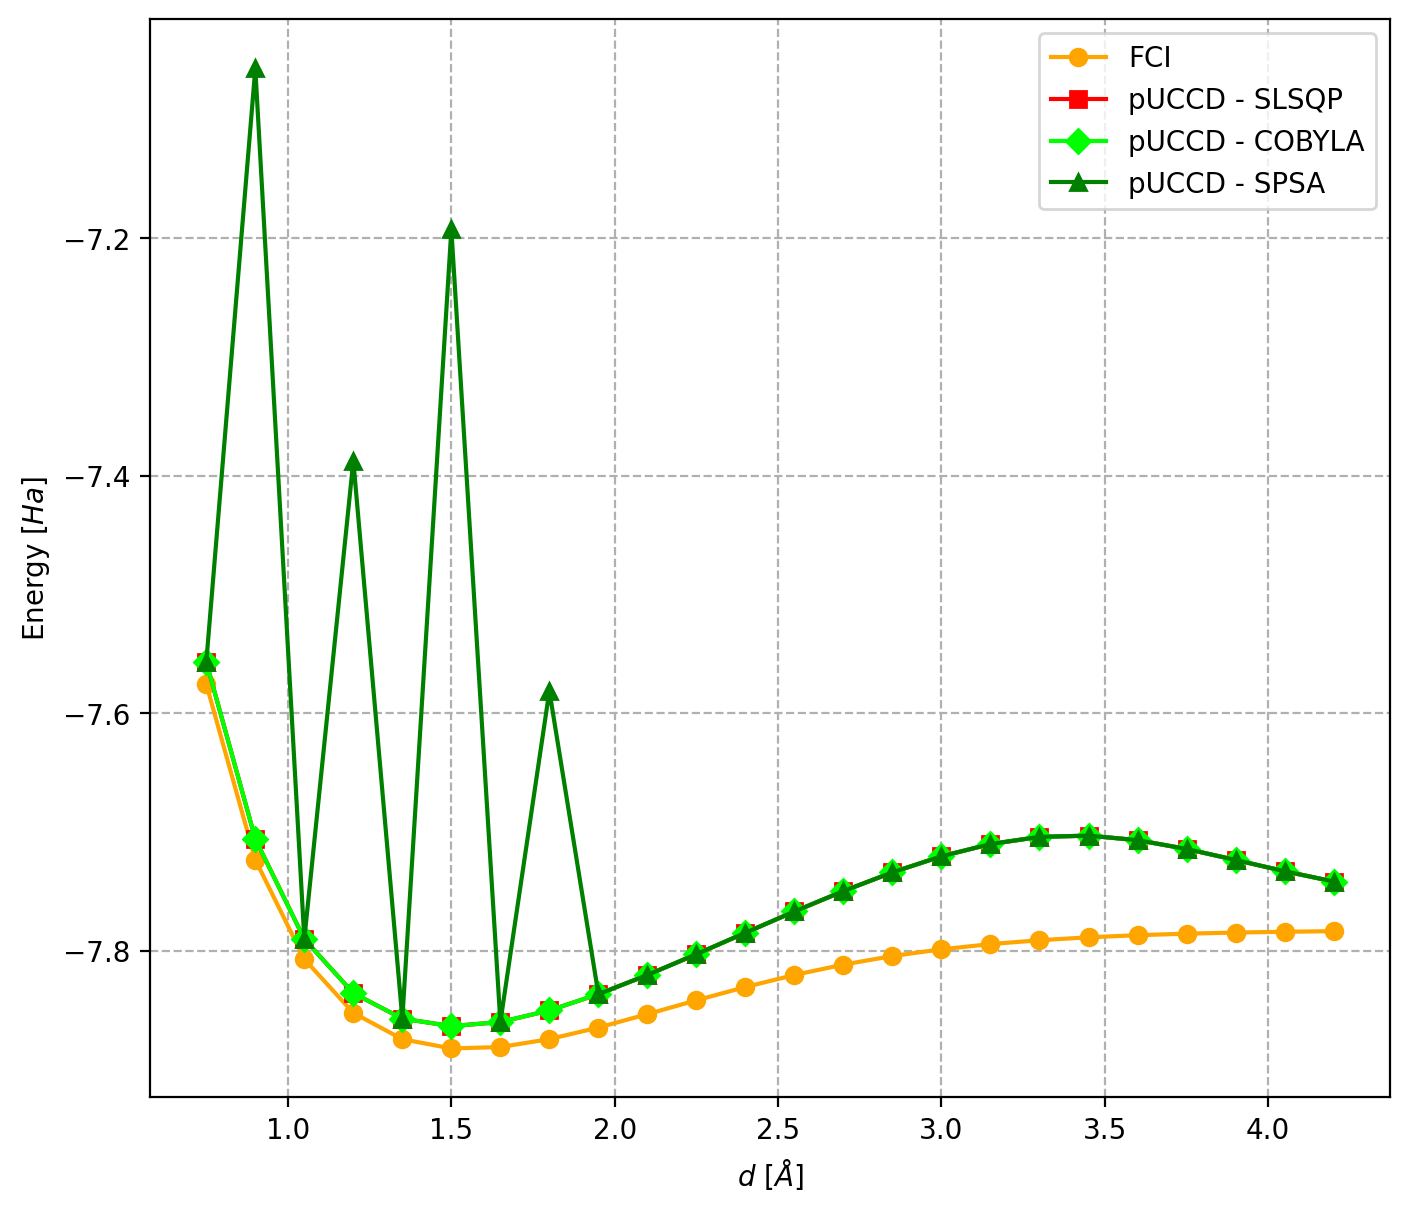
\includegraphics[width=.6\linewidth]{Immagini/Capitolo_3/LiH_optimizers.png}
    \caption{LiH: $q$-pUCCD con diversi ottimizzatori.}
    \label{fig:LiH-ottimizzatori}
\end{figure}

	
COBYLA e SLSQP convergono a risultati simili nelle energie calcolate, mentre SPSA, a parità di iterazioni, non riesce a raggiungere la convergenza. Questo può dipendere dal fatto che SPSA è ottimizzato per lavorare in condizioni rumorose, dove fornisce maggiore stabilità.





